\documentclass[12pt]{article}
\usepackage{amsmath}
\usepackage{amsfonts}
\usepackage[utf8]{inputenc}
\usepackage{default}
\usepackage[margin = 1.5in]{geometry}
\usepackage[round]{natbib}
\usepackage{graphicx}
\usepackage{rotating}
\usepackage{appendix}
\usepackage{palatino}
%\usepackage{wrapfig}
%\usepackage[nolists]{endfloat}

\title{Conspicuous Consumption in the United States and China}
\author{David Jinkins
    \thanks{I thank the National Science Foundation EAPSI program for support.  I would also like to thank Jonathan Eaton, Ed Green, Jim Tybout, Venky Venkateswaran, Yaohui Zhao, and the participants in the Penn State I/O and Trade reading groups for helpful comments. Remaining errors are my own.}
}
\date{July 4, 2014}

\begin{document}
\maketitle

\begin{abstract}
I develop a model of conspicuous consumption to empirically measure the importance of peer beliefs to Americans and Chinese.  In the model, a consumer cares not only about the direct utility she receives from consumption, but also about the way her consumption pattern affects her peer group's belief about her well-being.  I estimate the model on household budget surveys. According to model estimates, a Chinese consumer cares 20\% more than an American consumer about peer beliefs.  The absolute size of the conspicuous consumption motive is significantly smaller than that found in previous literature.  I use the estimated model to evaluate the welfare effect of the 1990-2002 American luxury tax on automobiles.  The luxury tax benefited nearly all Americans a small amount, but hurt the small fraction of consumers who love automobiles the most. \end{abstract}

\section{Introduction}

I wear a Seiko automatic watch.  Over the course of a month, it picks up about five minutes.  I knew it would do this before I bought it from reading online reviews, but even so I purchased it for about \$100 a few years ago.  At the time, I could have picked up a much less expensive digital Casio from Wal-Mart which would have run more reliably, been easier to read, and been more water resistant.  On just about any measure of watch performance the Casio would have outrun the Seiko, and yet there is the relatively expensive Seiko on my wrist.

When buying a car or a suit, a consumer considers how her social group will view the new purchase.  In addition to evidence from personal introspection, I will cite some papers below which find reduced form evidence of such consumer behavior. This paper adds to the empirical literature on conspicuous consumption by developing and estimating a partial-equilibrium heterogeneous-agent structural model in which a consumer's peers infer his wealth after observing a subset of his purchases.  Inference about welfare by his peer group causes a consumer to distort his consumption toward the purchase of visible goods.

This paper adds to the recent empirical literature on conspicuous consumption by developing and estimating a new structural model.  To identify the strength of the motive to conspiciuously consume, previous literature has either relied on strong assumptions about the functional form of utility or arbitrary assumptions about the way in which observable consumption enters utility.\citep{heffetz2011, perez2013measuring}.  In the model developed below, households are allowed to have heterogenous, non-homethetic preferences.  A peer group forms beliefs about the household's welfare based on the observable part of the household's consumption.  The household cares about these peer group beliefs, and takes them into account when chosing how to allocate its income.  In order to identify this more flexible model, I use differences in the perception of the observability of good categories across demographic groups, along with differences in how these demographic groups spend their incomes. The estimation uses both a survey on the relative visibility of different categories of goods, and household-level consumption expenditure data.  As it is used to calculate purchasing power, expenditure data is available for many countries and time periods.  This is primarily a \emph{measurement} paper.

I estimate the model separately using American and Chinese consumption expenditure data.  MOTIVATE HERE WHY WE MIGHT CARE ABOUT COMPARING THE US AND CHINA.  The estimated model fits the data well.  I find that the Chinese consumers care 20\% more than American consumers about peer group beliefs.  Using the estimated model, I find that the 1990-2002 American luxury tax on automobiles had a small but positive welfare effect on all but around 2 in 10,000 American households.  The households hurt by the tax were gearheads that derived a large amount of pleasure from automobile purchases.

In this paper as well as the literature I am following, a consumer considers peer group belief an end in itself.  I put peer group belief about welfare directly into the utility function.  Some might argue that people only care about peer group beliefs as the means to an ultimate consumptive end--wearing a nice watch makes people trust you more, so you are more likely to get a loan or secure a business deal.  I am sympathetic to this point of view, and this sort of signaling is doubtless going on to some degree.  The two points of view about peer beliefs are complementary.  From a long perspective, our brains might have been selected to care about peer group beliefs precisely because good standing makes successful reproduction more likely. In this case, the utils we get from positive peer group beliefs are an evolutionary rule of thumb.\citep{RobsonSamuelson2010}

There are several strands of empirical literature that support the presence of a peer belief component in the utility function.  Consider the ultimatum game in which one player proposes a split of a sum of money, and the other player decides whether to accept or reject.  If the second player accepts, the money is allocated according to the split. If the second player rejects, neither player gets anything.  There is a long and robust experimental literature showing that if people only care about immediate monetary payoffs, the splits they propose are too fair.  Researchers have been careful to pair subjects who do not know each other and are unlikely to have interaction after the experiment, and the result still holds.  One explanation is that there is some sort of social component in the utility function. \citep{FehrSchmidt1999,BoltonOckenfels2000}  A second defense comes from the literature on self-reported happiness and relative wealth.  \citet{Luttmer2004} finds that relative wealth compared with neighbors has a robust positive correlation  with self-reported happiness, controlling for absolute wealth level.  It seems hard to explain this fact without some sort of social component in the utility function.  If, however, the reader is not convinced that there is a fundamental social belief component in the utility function, he may think of this paper as estimating a reduced form of a more complicated dynamic game.  
This paper adds to the empirical literature on conspicuous consumption.\citep{Blochetal2004,Charlesetal2009,MoavNeeman2010,MoavNeeman2012}  I extend work by \citet{Heffetz2011}, who conducts a telephone survey in the United States to determine the visibility of consumption goods.  Heffetz analyzes household budget survey data, and finds evidence that the relatively visible goods identified by the survey are being used as a means to signal income.  To my knowledge, the only other structural estimation of a utility function including conspicuous consumption is \citet{perez2013measuring}.  Perez-Truglia follows earlier literature in using a two-good functional form, and a variety of specifications for how non-market goods like status enter utility.  My specification below differs from Perez-Truglia's in a few important ways.  Some cosmetic differences include that I allow for individual level preference heterogeneity and estimate a many good utility function.  Any good can be used for signaling in my model, while in Perez-Truglia's model cars and clothes are the visible goods.  More substantively, while Perez-Truglia is focused on the provision of unobservable non-market goods (status), I assume that society cares only about an individual's unobservable welfare.  This allows me to consider peer-group beliefs as an equilibrium outcome, rather than assume a functional form for the provision of a non-market good.  In his framework, Perez-Truglia finds that a tax on luxury goods can create welfare gains significantly larger than those I find in my estimation.

There is a relatively large and old related literature estimating what are known as interdependent preferences.  Beginning with James Duesenberry's 1949 doctoral thesis,\citep{Duesenberry1949} researchers have theorized that the consumption of neighbors affects own demand.  A typical econometric model in this literature lets household demand parameters depend linearly on the average of the consumption of a reference group. A relationship between neighbor consumption and own consumption is taken to mean that preferences are interdependent.  The literature, however, does not take a stand on why consumption neighborhood consumption should be linked in this particular way.

Structural estimation allows me to both measure the motive for conspicuous consumption across countries, and to calculate the welfare gains from an excise tax on a visible good category.  A well-designed excise tax can raise nearly everyone's welfare.  If income were directly observable by the peer group, there would be no reason to distort consumption towards visible goods and welfare would be higher than in the incomplete information world.  One way to get people closer to the complete information allocation is to raise the price of the visible good, and then redistribute the proceeds of the tax.  Loosely speaking, the rich are better off because they distort consumption less, and the poor are better off because they are getting a subsidy from the rich.  If people care deeply about peer group belief, then the welfare gains from this sort of tax can be large.\footnotemark\footnotetext{Signaling distortions are particularly worrying when considering the economic lives of the poor.  A recent study reports that in parts of India, the \emph{median} household making under a dollar a day spends 10\% of its income on festivals--this while 43\% of such households did not have enough to eat throughout the year.\citep{BanerjeeDuflo2007}} 


\section{An Empirical Model of Conspicuous Consumption}

There is a finite set of goods $G$.  Each good has an exogenous price $p_g$.  There is a continuum of consumers $I$. For each consumer, nature draws a income $w_i$, a preference type $\boldsymbol{\gamma}_i$, and an observation type $t_i \in G$.  A consumer allocate his income to goods in order to maximize his utility.  Following previous literature on conspicuous consumption \citep{Heffetz2011,Ireland1994}, I assume a consumer's utility function consists of two additively separable parts.

\begin{equation}
    \label{eq:metautil}
    U(\mathbf{C}_i,\boldsymbol{\gamma}_i,t_i) = (1-\alpha) u(C_i,\boldsymbol{\gamma}_i) + \alpha\  u(C_b(c_{t_i},\boldsymbol{\gamma}_i,t_i),\boldsymbol{\gamma}_i)
\end{equation}

The first term on the right-hand side of \eqref{eq:metautil} is a fundamental utility $u:\mathbb{R}_+^{I}\rightarrow\mathbb{R}$.  
Fundamental utility describes the pleasure a consumer gets directly from consuming a bundle of goods.
The second term is the belief of a consumer's peer group over his utility.  Peer group belief over the utility level of consumer $i$ is based on his expenditure on good category $t_i$.  $C_b$ maps consumption of the observable good, observation type, and preference type to the unobservable full consumption vector.  The preference type and observation type of consumer $i$ are known to his peer group.\footnotemark\footnotetext{The peer-group infers the one-dimensional income of a consumer from the one-dimensional observed consumption choice of the observable good.  If I allow for more than one observed good, then one-dimensional would be inferred from multi-dimensional consumption.  As in a typical multi-dimensional screening model, the equilibrium will be driven by beliefs off the equilibrium path and there will be many possible equilibria.}

\subsection{Equilibrium Concept}

An equilibrium is a social belief function $C_b$ and a consumption function $C$ on $(W,\Gamma,G)$ such that:
\begin{enumerate}
    \item For each consumer type $(w_i,\boldsymbol{\gamma}_i,t_i), \ C(w_i,\boldsymbol{\gamma}_i,t_i)$ solves the consumer's problem.
    \item For each consumer types $(w_i,\boldsymbol{\gamma}_i,t_i), \ C(w_i,\boldsymbol{\gamma}_i,t_i) = C_b(C(w_i,\boldsymbol{\gamma}_i,t_i)_{t_i},\boldsymbol{\gamma}_i,t_i).$
\end{enumerate}
The first condition says that a consumer chooses an optimum consumption bundle, and the second condition says that Consumer $i$'s peer group learns his true type.

\subsection{Specializing to Cobb-Douglas}

Let the fundamental utility function be Cobb-Douglas:
\[u(\mathbf{C}, \boldsymbol{\gamma}) = \sum_{g=1}^{G} \gamma_g \ln(c_g)\]
The model can then be written as a generalization of the Heffetz model to many goods and preference heterogeneity.\footnotemark\footnotetext{ In the Heffetz version, there are only two goods, one visible and the other invisible to society. In my version, there is one visible good for each observation type, and all the other goods are invisible.}
In what follows I drop subscripts for Consumer $i$ to simplify notation. Let $t \in G$ be Consumer $i$'s observation type, and let $c_{t}^*$ be Consumer $i$'s equilibrium consumption of the visible good.  Equilibrium demand for good $g\neq t$ conditional on spending on the visible good is the standard Cobb-Douglas constant expenditure share:
\begin{equation}
    \label{eq:opt_cobb}
    p_g c_g^* = \gamma_g\left(\sum_{j\neq t} \gamma_j\right)^{-1}\left(w-p_t c_t^* \right)
\end{equation}

Using the demands, we can write the utility function as a function of visible good consumption.
\begin{equation}
    \label{eq:ufun}
    U(c_t) = (1-\alpha) \left(\hat{\gamma} \ln \left(w-p_t c_t\right) + \gamma_t \ln \left(c_t \right)\right) + \alpha \left(\gamma_t \ln \left(s(c_t)\right) + \gamma_t \ln \left(c_t\right) \right) + \zeta(\mathbf{p},\boldsymbol{\gamma})
\end{equation}
Here $\hat{\gamma} = \sum_{g\neq t} \gamma_g$ and $\zeta(\mathbf{p},\boldsymbol{\gamma})$ is a constant which depends only on utility parameters and prices.  The single-valued function $s(c_t)$ is the belief of the peer group about spending on non-visible goods $w-p_t c_t$. 

Consumer $i$ maximizes utility function \eqref{eq:ufun} subject to his budget constraint.  The first order condition for an interior solution to his problem can be written:
\begin{equation}
	\label{foc}
s'(c_t^*) = \frac{1}{\alpha}\left( \left( 1-\alpha\right) p_t - \frac{\gamma_t}{\hat{\gamma}}\frac{s(c_t^*)}{c_t^*}\right)
\end{equation}
This differential equation has the solution:
\begin{equation}
	\label{eq:difsol}
    s(c_t^*) = \frac{\hat{\gamma}\left(1-\alpha\right)}{\gamma_t +\alpha \hat{\gamma}} p_t c_t^* +  \frac{\hat{\gamma} \alpha }{\gamma_t + \alpha \hat{\gamma}} \underbar{W}\frac{p_t c_t^*}{p_t \underbar{c}}^{-\frac{\gamma_t}{\alpha \hat{\gamma}}}
\end{equation}
The constant in the solution \eqref{eq:difsol} is pinned down because the lowest possible income type $\underbar{W} > 0$ has no reason to signal in a separating equilibrium.  His expenditure on the visible good $\underbar{c}$ is the fraction $\gamma_t / \sum_j \gamma_j$ of his income.  As one might expect, the function $s$ is jointly homothetic in $c_t^*$ and $\underbar{W}$.

Define equilibrium expenditure share on the visible good category $r = p_t c_t^* / w$, the ratio $\gamma = \gamma_t / \hat{\gamma}$, and normalized income $\hat{w} = \underbar{W} / w$.  Substituting in for the $s$ function and dividing by income, we have a simplified equilibrium condition:

\begin{equation}
	\label{eq:eq_cond}
    (1 - r)(1 + \frac{\gamma}{\alpha}) = \frac{\left(1-\alpha\right)}{\alpha} r +  \left(r\left(1 + \gamma^{-1}\right)\right)^{-\frac{\gamma}{\alpha}}\hat{w}^{1+\frac{\gamma}{\alpha}}
\end{equation}

\section{Description of Data and Sources}
This project requires two types of data.  We need household-level consumer expenditure data, and we need information about how visible different good categories are relative to each other.  Household expenditure data is widely available from national statistical agencies.  Information on the visibility of different good categories is taken from a survey conducted in \citet{Heffetz2011}.

\subsection{Household Expenditures}
American household expenditure data is taken from the National Bureau of Economic Research.\citep{NBERCEX2011}  This data set is publicly available, and features a large random sample of American household consumption decisions for selected years between 1981 and 2002.  In addition to detailed information on household income and expenditures, the NBER data set contains demographic data on household members such as age, race, sex, and location.
There are 47 good categories available in the NBER data set.
Following \citet{Heffetz2011} exactly,\footnotemark\footnotetext{Heffetz was kind enough to give me his STATA code.} I aggregate into 29 expenditure categories.
The cleaned NBER data set contains 160,617 household observations across 18 years.

Households display widely varying consumption behavior.  Figure \ref{fig:exp_shr} is a scatter plot the 2001 log budget shares by log expenditures.  Representative household models in the literature such as those by Heffetz and Ireland cannot replicate this heterogeneity.\footnotemark\footnotetext{\citet{Heffetz2011} contains a discussion of this issue.} The heterogeneous preference model estimated in this paper can potentially match the noise observed in the data.

\begin{figure}
	\centering
		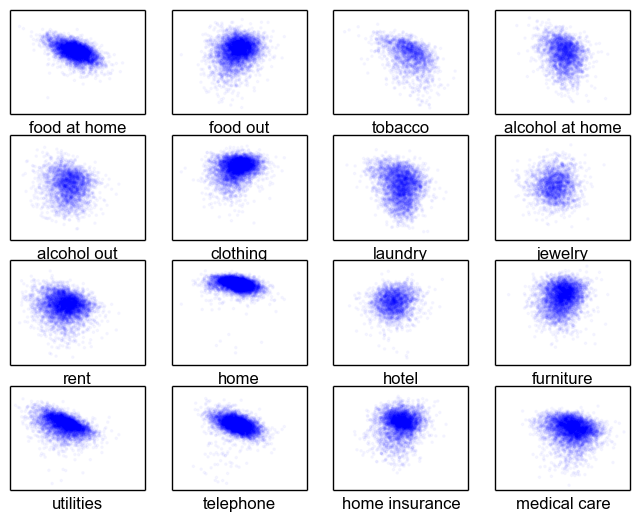
\includegraphics[scale=1]{pics/shr_plot.png}
	\caption{Log expenditure shares (y) by log expenditure (x)}
	\label{fig:exp_shr}
\end{figure}

For the Chinese household expenditures, I use publicly available data from the Chinese Household Income Project (CHIP). \citep{CHIP2002} Like the American household expenditure data, the CHIP data is comprised of repeated cross-sections of Chinese households.  In this study I use urban households surveyed in 1995 and 2002 for a total of 13,767 observations.  I use 14 good categories which correspond to aggregates of those in the American household expenditure survey.   Table \ref{tab:chncons} details the link between the American and Chinese expenditure data.
\begin{table}
    \centering
    \footnotesize
 \begin{tabular}{llll}
        \hline \hline
        US Cat & 1995 Chn Cat & 2002 Chn Cat & Chn Cat Name  \\
        \hline 
        Fdh,Fdo     & h27        & e1-e152-e153 & Food-Cig.-Alcohol\\
        Alh,Alo     & h30-h31    & e153         & Alcohol\\
        Cig         & h31        & e152         & Cigarettes\\
        Bks         & h37        & f631         & Textbooks\\
        Edu         & h38 to h42 & f63-f631     & Education-Textbooks\\
        Bus,Car\footnotemark{}    & h44        & f514         & Transportation\\
        Utl         & h45 to h46 & f72          & Water,Elec.,Fuel\\
        Tel         & h47        & f522         & Communication\\
        Clo,Jwl     & h32        & f2           & Clothes\\
        Ot1,Ot2     & h33        & f6-f63       & Entertain.\\
        Fur,Lry,Brb & h34,h36    & f3           & HomeEquip.,Facil.,\\
        Med,Lin     & h48        & f4           & Health\\
        Hom,Htl     & h64        & f71          & Housing\\
        Fee,Cha     & h35        & f8           & Misc.Goods\\\hline
 \end{tabular}
    \caption{US-China Consumption Category Correspondence}
    \label{tab:chncons}
\end{table}

\footnotetext{Air, Gas, Cmn, Cin}

\subsection{Visibility Indexes}
Data concerning the visibility of good categories is taken from \citet{Heffetz2011}.  
Heffetz bases the index on randomized telephone surveys conducted in the United States in several waves around 2004.
Survey respondents were asked how long it would take them to notice if a new acquaintance similar to themselves spent more than average on a particular good category.
Respondents chose from five time periods ranging from almost immediately to almost never.
Basic demographics similar to those in the consumer expenditure survey were also recorded for respondents.

From the survey responses, Heffetz creates indexes, called vindexes, between zero and one for each category of goods by averaging over survey results. 
A higher vindex value implies that a good category is more visible. 
A result of this aggregation methodology is that the index is cardinal rather than ordinal.  Two goods with similar index values are similar in visibility.  Details on the implementation of the survey and calculation of the index are available in the original paper.
Table \ref{tab:vintab} in the appendix presents vindex survey data.

As I do not have a vindex equivalent for China, I use the aggregated American vindex data for the Chinese estimation. Since there are fewer good categories in the Chinese data, I collapse the American vindex by taking the mean over aggregated good categories.

\section{Discussion of Model Identification}

We are interested in $\alpha$, the weight given to the peer belief part of the utility function.  The key identification issue is that, for a fixed $\alpha$, \emph{any} consumption bundle can be rationalized by a particular set of utility function parameters $\boldsymbol{\gamma}_i$.  In order to separate preferences and conspicuous consumption, we need to take a stand on how utility parameters might be distributed.  One natural assumption is that most people's preferences are broadly similar.  To operationalize this idea, I assume that preferences for each household and each good category are independently drawn from lognormal distributions.  In addition, to rationalize zero expenditure in a good category I assume that with some probability a consumer doesn't derive any pleasure from consumption of a particular category ($\gamma_{ig} = 0$).

A second challenge is that the Cobb-Douglass base utility assumption implies that there are no luxury or inferior goods.  Absent any conspicuous consumption, expenditure shares are constant as household  income increases.  Figure \ref{fig:exp_shr} shows that expenditure shares are changing on average as household income increases.  The combination of Cobb-Douglass utility and changing expenditure shares in principle identifies $\alpha$ in the model.

The Cobb-Douglass assumption is too strong, however.  I want to allow a good like ``food at home'' to be inferior even without conspicuous consumption effects.  To do this, I allow the location of the distribution of utility parameters to drift as a function of normalized income.  In particular, the location parameter $\hat{\mu}_g(w_i)$ of the lognormal distribution for good category $g$ is given by \eqref{eq:adj_util}.

\begin{equation}
    \label{eq:adj_util}
    \hat{\mu}_g(w_i) = \psi_g \ln \left(\frac{w_i}{\underbar{W}}\right) + \mu_g
\end{equation}

This 'money-in-the-utility-function' specification is somewhat ad hoc, but it allows us to keep the simple equilibrium condition \eqref{eq:eq_cond} as well as allowing for rich evolution of expenditure shares with income.  This distribution of utility parameters also breaks the simple identification of $\alpha$ from the correlation of household expenditure shares and income.

In order to regain identification, I use differences in observed vindexes across demographics.  I assume that all utility parameters $\boldsymbol{\gamma}_i$ are drawn out of the same distribution, but observation types $t_i$ are drawn with probability weighted by an individual's demographic specific vindex.  The size of differences in average consumption between demographic groups are then informative about the weight $\alpha$ of peer group beliefs in the utility function.

In the United States I use visibility indexes for eight different demographic types of household.  One dimension of differentiation is the age of the survey respondent (over/under age 40). The other dimension of differentiation is region in the United States (Northeast, Midwest, West, and South).  The visibility probabilities are taken directly from Heffetz and normalized so that they sum to one.  Table \ref{tab:dem_vin} in the appendix characterizes observation-type probability distributions for the demographic groups.

I have only a single Chinese demographic category, so when estimating Chinese preference parameters I cannot use an identification strategy based on differences across demographic groups.  MORE DISCUSSION OF WHETHER THIS IS A BIG PROBLEM!  In the Chinese estimation, I take the $\psi_g$'s in equation \eqref{eq:adj_util} as data from the American estimation.  This assumption implies that luxury and inferior good categories are the same in both China and the United States.  Deviations from Chinese expenditure share trends along with vindex probabilities identify $\alpha$.

\section{Estimation Procedure} 


In order to estimate the parameter of interest $\alpha$, we must jointly estimate the observation type of each household and four preference distribution parameters for each good category.  This is a large problem, so I split the estimation into two steps by using a 'hard' expectation maximization algorithm.  In the first step (maximization), I condition on the observation type of each household and update $\alpha$ and preference distribution parameters.  In the second stage, I take $\alpha$ and the preference distribution parameters as given and find the most likely observation type of each household (expectation).  The algorithm stops when there is no change in $\alpha$.\footnote{Intuitively this algorithm converges because in each step the likelihood must weakly increase.  As with other expectation maximization algorithms, the algorithm used here will stop at either a local maximum, or a saddle point.} 

\subsection{Maximization: Updating $\alpha$ and Preference Distribution Parameters} 

\subsubsection{Overview}
In the maximization step, I condition the likelihood function on the observation type $t_i$ of each household and update $\alpha$ and lognormal preference distribution parameters $\mu_g$, $\sigma_g$, income-scaling parameter $\psi_g$, and a zero probability $z_g$.  The outer structure of the maximization step uses a numerical optimizer to maximize the conditional likelihood over $\alpha$, and to treat the likelihood-maximizing preference parameters and preference distribution parameters as functions of $\alpha$.  Given $\alpha$, the preference parameters $\boldsymbol{\gamma}_i$ of each household can be calculated using observed consumption shares.  Once we have preference parameters for each household, we can analytically calculate the most likely lognormal preference distribution and zero parameters.

\subsubsection{Recovering Household Preference Parameters Given $\alpha$}
\label{sec:upd_prefs}

Taking observation type $t_i$ and $\alpha$ as given, there is a mapping from observed consumption shares directly to household preference parameters.  Consider a household of observed income type $w$, observed consumption vector $C$, and observation type $t$.  Rearranging \eqref{eq:opt_cobb}, $\gamma_g$ for $g\neq t$ are given by :
\begin{align}
	%\label{eq:sgd}
	p_gc_g &= \frac{\gamma_g}{\sum_{g\neq t}\gamma_g}  \left(w-  p_t c_t\right) \nonumber \\
	%\label{eq:sgdsol}
	\gamma_g &= \frac{p_g c_g}{\left(w- p_t c_t\right)} \sum_{g\neq t}\gamma_g \nonumber \\
	\label{eq:gamsol}
	\gamma_g &= \frac{p_g c_g}{\left(w- p_t c_t\right)} 
\end{align}

We can solve for the 28 non-observation type $\gamma_g$'s up to a scaling factor $\sum_{g\neq t}\gamma_g = 1$.  Using \eqref{eq:gamsol} and the equilibrium condition \eqref{foc} we can then solve for $\gamma_t$.  Unfortunately, \eqref{foc} is non-linear and in principle needs to be solved numerically for each household.  To decrease estimation time, in practice I solve \eqref{foc} on a 1000 point grid of visible consumption shares and incomes, and then linearly interpolate to find household specific $\gamma_t$'s.

\subsubsection{Updating Preference Distribution Parameters}

Given $\alpha$ and household preference parameters $\boldsymbol{\gamma}_i$ for each household $i \in I$, the most likely zero probability $z_g^*$ for good category $g$ is the fraction of zero $\gamma_{ig}$'s:

\begin{equation}
    z_g^* = \frac{1}{\|I\|} \sum_{i} \mathbf{1}_{\gamma_{ig} = 0} \nonumber
\end{equation}

Let an upper bar denote sample means over non-zero $\gamma_i$'s, and let $m_i$ refer to normalized income, $m_i = w_i/\underbar{W}$.  The other likelihood-maximizing preference parameters are:

\begin{align}
    \psi_g^* &= \frac{\hat{\mbox{cov}}(\ln m, \ln \gamma)}{\hat{\mbox{var}}(\ln m)} \nonumber \\
    \mu_g^* &= \overline{\ln \gamma} - \psi_g^* \overline{\ln m} \nonumber \\
    \sigma_g^{2*} &= \overline{\left(\ln \gamma - \psi_g^* \ln m - \mu_g^*\right)^2}
\end{align}

\subsubsection{Full Conditional Likelihood Function}

I have shown how, given observation types, it is straight-forward to calculate preference parameters and likelihood maximizing preference distribution parameters as a function of $\alpha$.  Let $\phi$ be the log-normal probability density function.   The maximization step conditional log-likelihood function is given in \eqref{lik1}.  All preference parameters and preference distribution parameters are implicitly functions of $\alpha$.

\begin{equation}
	\label{lik1}
    l^1(\alpha) = \sum_{ig} \left(\mathbf{1}_{\{\gamma_{ig} = 0\}}\ln\left(z_g\right) + \mathbf{1}_{\{\gamma_{ig} \neq 0\}} \left(\ln\left(1 - z_g\right)+\ln \phi(\gamma_{ig},m_i|\mu_g,\sigma_g,\psi_g)\right)\right)
\end{equation}
Likelihood \eqref{lik1} is the objective function used by the numerical solver in the search for $\alpha$.  This completes the characterization of the maximization step in the algorithm.

\subsection{Expectation: Updating Observation Type $t_i$} 

Given the utility weight of social beliefs $\alpha$ and a set of preference distribution parameters, we find the most likely observation type for each household. Now preference parameters $\gamma_{ig}$ are a function of observation type $t$ and are calculated exactly as in Section \ref{sec:upd_prefs}. $\mathbf{v}_i$ is the household-specific vector of observation type probabilities.  Household $i$'s (unnormalized) probability of being observation type $t \in G$ is given by \eqref{lik2}.

\begin{equation}
    \label{lik2}
    l_i^2(t) = \ln(v_{it}) + \sum_{g} \left(\mathbf{1}_{\{\gamma_{ig} = 0\}}\ln\left(z_g\right) + \mathbf{1}_{\{\gamma_{ig} \neq 0\}} \left(\ln\left(1-z_g\right)+\ln \phi(\gamma_{ig}, m_i|\mu_g,\sigma_g,\psi_g)\right)\right)
\end{equation}
For each household, I assign the observation type giving the highest probability.  This concludes the discussion of the estimation routine.

\section{Results and an Application to an American Luxury Tax}
\label{sec:results}

Chinese care about 20\% more than Americans about social beliefs.  The weight of social beliefs $\alpha$ in American utility is 0.027 with standard error $1\times10^{-4}$.  In Chinese utility, the weight of social beliefs is 0.033 with standard error 0.001.  Standard errors are bootstrapped by repeatedly redrawing from the data and reestimating the model.  All estimated parameters are presented in Appendix \ref{det_res}.

The model is capable of simulating data similar to the real data set. Figure \ref{fig:shares_fake} is a scatter plot of simulated US data, superimposed on top of the scatter plots of the actual US data in figures \ref{fig:exp_shr}.
\begin{figure}
	\centering
		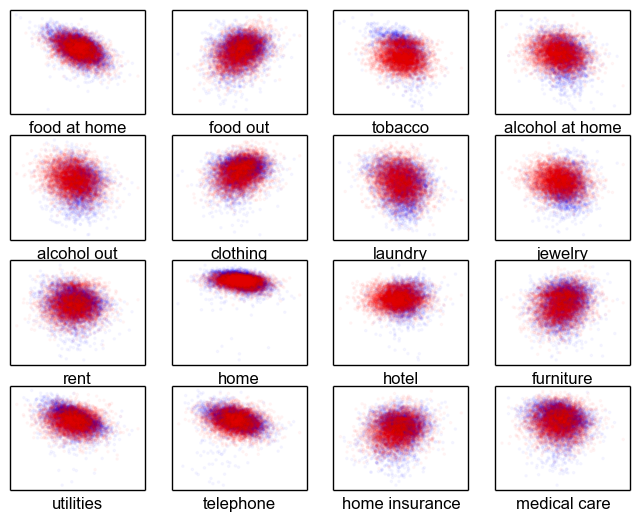
\includegraphics[scale=1]{pics/shr_plot_sim.png}
	\caption{Log expenditure shares (y) by log expenditure (x), sim=red, dat=blue}
	\label{fig:shares_fake}
\end{figure}
The estimation also does well fitting observation types.
The observation type distribution (for a particular demographic) should be the same as the vindex probability distribution.
Figure \ref{fig:vinmatch} is a scatter plot of the vindex probabilities and the estimated observation type densities.  Each point is labeled with the relevant good category, and the colors represent different demographic types (region and age). Although there is not a perfect correlation between vindex probabilities and observation type frequencies, there is a clear trend in the right direction.  The model misses the most on good categories ``car'' and ``jewelry''.  I suspect the problem is that these are durable goods, so that a single year of expenditure is a poor reflection of average expenditure in those categories.
\begin{figure}
    \centering
	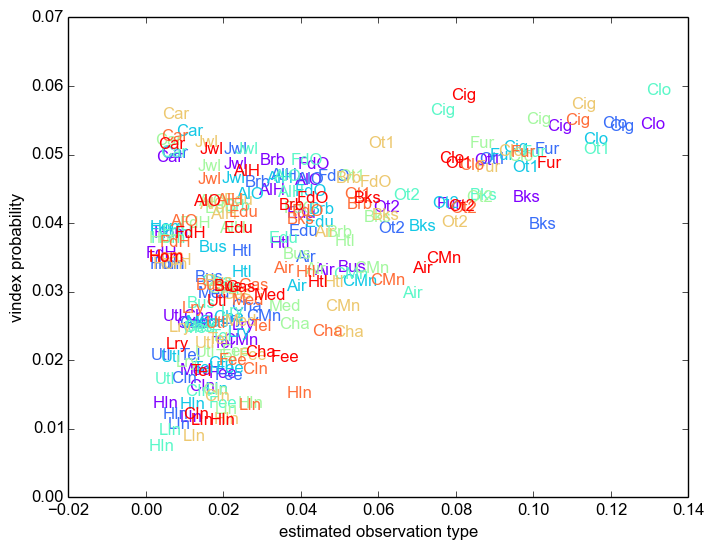
\includegraphics[scale=.8]{pics/obs_vin_scat.png}
    \caption{Estimated observation type frequencies vindex probabilities, by demographic}
    \label{fig:vinmatch}
\end{figure}

HOW ARE MY RESULTS IN LINE WITH HEFFETZ?

ROBUSTNESS: IS AGGREGATION CAUSING THE DIFFERENCE BETWeeN CHINESE AND AMERICANS

\subsection{Policy Analysis: Luxury Tax}

BETTER APPLICATION INVOLVING BOTH US AND CHINA.

In the model developed above, a consumer distorts his full-information utility-maximizing consumption bundle in order to signal his income.  The signal is on expenditures, however, not on physical goods.  In principle, a social planner could impose a sales tax on a highly visible good category in order to reduce physical consumption.  In the real world, such a tax is known as a luxury tax.  In this section I consider the welfare implications of one such tax scheme, an American luxury tax on automobiles.

\subsubsection{Application: Welfare Effect of US Automotive Luxury Taxes}

In 1990, President George H.W. Bush signed the Omnibus Budget Reconciliation Act into law.\footnotemark\footnotetext{Some readers might remember that this act proved television to be a poor medium for lip-reading.}  The OBRA contained a provision for a luxury tax on automobiles, as well as jewelry, furs, yachts, and personal aircraft.  The tax on autos was 10\% of the price exceeding \$30,000.  As one might imagine, the luxury tax did not go over well at campaign fundraisers and was repealed in 1993 for all goods except automobiles.\footnotemark\footnotetext{A cynical political realist might observe that luxury vehicles are often imported from Europe.}  Congress finally scrapped the auto tax in 2002.

In this section, I measure the welfare effects of a 10\% tax on automobiles, redistributed lump sum as a proportion of wealth.  Redistributing the tax proportionally to wealth conveniently abstracts from the welfare effect of a transfer from the rich to the poor.  In addition, taxes redistributed this way change neither the individual nor aggregate fraction of wealth optimally allocated to any particular good category, as relative wealth remains unchanged.

My luxury tax will be 10\% of spending on automobiles.  Let $\tau = 0.1 / 1.1$ be the fraction of spending on autos taken by the government, let $s$ be the fraction by which the government increases wealth levels, let $l_i$ be the equilibrium fraction of auto expenditure in consumer $i$'s total expenditures, and let $L$ be the aggregate fraction of spending on automobiles.  Condition \eqref{eq:lux_bb} balances the budget.

\begin{align}
    (1 + s) \tau \sum_i w_i l_i &= s \sum_i w_i \nonumber \\
    s &= \frac{\tau \sum_i w_i l_i}{\sum_i w_i - \tau \sum_i w_i l_i} \nonumber \\
    \label{eq:lux_bb}
    s &= \frac{\tau L}{1 - \tau L}
\end{align}

Welfare change under the tax scheme is as in \eqref{eq:us_wel_change}.

\begin{equation}
    \label{eq:us_wel_change}
    \Delta u_i = \sum_{g\in G} \gamma_{ig} \ln(1 + s) + \sum_{g\in l} \gamma_{ig} \ln (1 - \tau)
\end{equation}

Using \eqref{eq:lux_bb}, it can be shown that $\ln(1+s) + \ln(1 - \tau) \leq 0$ with the inequality strict when the aggregate share of spending on automobiles $L$ is less than one.  Thus, it is impossible to have a truly Pareto tax scheme.  That is, it is always possible that some unlucky consumer will draw all zero $\gamma_{ig}$'s in non-luxury good categories, ensuring he will be harmed by a luxury tax.  We can, however, potentially design taxes which benefit all but a very small fraction of consumers.

The relationship between $\alpha$ and the tax scheme here is through the share of expenditures households spend on automobiles, a relatively visible good category.  Since many households have automobiles as an observation type, fixing preference parameters and the tax level $\tau$, the higher is $\alpha$ the higher will be government subsidies $s$ to consumers.

Figure \ref{fig:wel_change_10} displays a histogram of welfare changes resulting from a 10\% luxury tax, calculated for one million American households simulated using estimated model parameters from Section \ref{sec:results}.  About 0.02\%, or two in 10,000 households are harmed by the auto luxury tax.  The vast majority of households benefit from the automobile luxury tax.  In contrast, a similar 10\% sales tax on food at home harms 90\% of households.

\begin{figure}
    \centering
	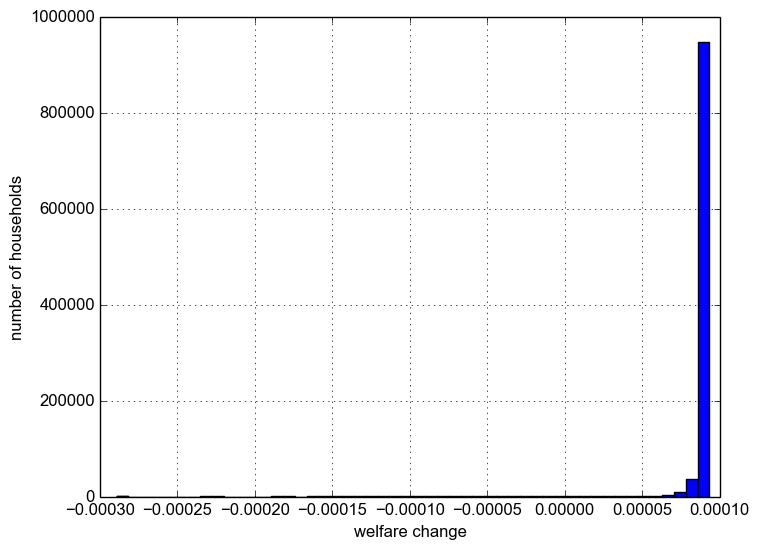
\includegraphics[scale=.6]{pics/tax_hist_Car10.png}
    \caption{Histogram of welfare changes from a 10\% luxury auto tax}
    \label{fig:wel_change_10}
\end{figure}

\section{Summary}
I develop a structural conspicuous consumption model with preference heterogeneity estimable from widely available consumption expenditure data.  In an application, I show how the estimated model can be used to measure the welfare implications of a tax on luxury goods.

The results of the estimation show that:
\begin{enumerate}
    \item Peer group belief plays a small but non-zero role in overall consumption decisions.  American and Chinese consumers value peer group belief under five percent as much as they value the direct utility from consumption.
    \item Chinese consumers value peer group belief 20\% more than American consumers.
    \item Simple luxury taxes can lead to small welfare gains for nearly all households.
\end{enumerate}

The strongest assumption in the model is that a household's peer group sees only consumption expenditures on one good category.  While a single-dimensional signal generates the unique and simple equilibrium solution to the model, it is clearly counterfactual.  In the real world, one's peer group sees a full, noisy vector of consumption expenditures.  An earlier version of this paper had a model with this feature, but estimation involved numerically calculating a thirty dimensional integral for each consumer for each parameter trial.  Future research might focus on relaxing this stark assumption about the observability of consumption.

\newpage

\bibliographystyle{apalike}
\bibliography{/home/veryshuai/Documents/bib/biglist.bib}

\newpage

\appendix

\section{Vindex Tables}
\label{sec:vin_tables}

\begin{table}[!ht]
    \centering
\begin{tabular}{lcc}
	\hline\hline
	Category & Vindex & SE \\
	\hline 
cigarettes       & 0.76 & (0.014) \\
cars             & 0.72 & (0.012) \\
clothing         & 0.70 & (0.013) \\
furniture        & 0.68 & (0.012) \\
jewelry          & 0.67 & (0.015) \\
recreation 1     & 0.66 & (0.012) \\
food out         & 0.61 & (0.012) \\
alcohol home     & 0.60 & (0.014) \\
barbers etc      & 0.60 & (0.014) \\
alcohol out      & 0.59 & (0.014) \\
recreation 2     & 0.57 & (0.013) \\
books etc        & 0.57 & (0.013) \\
education        & 0.56 & (0.014) \\
food home        & 0.51 & (0.014) \\
rent/home        & 0.49 & (0.016) \\
cell phone       & 0.46 & (0.016) \\
air travel       & 0.46 & (0.014) \\
hotels etc       & 0.45 & (0.013) \\
public trans     & 0.44 & (0.015) \\
car repair       & 0.42 & (0.014) \\
gasoline         & 0.39 & (0.016) \\
health care      & 0.36 & (0.014) \\
charities        & 0.34 & (0.014) \\
laundry          & 0.33 & (0.015) \\
home utilities   & 0.31 & (0.015) \\
home phone       & 0.29 & (0.015) \\
legal fees       & 0.26 & (0.013) \\
car insur        & 0.22 & (0.014) \\
home insur       & 0.16 & (0.012) \\
life insur       & 0.16 & (0.011) \\
underwear        & 0.12 & (0.011) \\
\hline
\end{tabular}
\caption{Aggregate Vindex}
\label{tab:vintab}
\vspace{-2in}
\end{table}

\begin{table}[!ht]
    \centering
    {\footnotesize
    \begin{tabular}{lllllllll}
        \hline\hline
        & \multicolumn{4}{c}{Interviewee age under 40} & \multicolumn{4}{c}{Interviewee age over 40}\\
            & NEast & South & MWest & West  & NEast & South & Mwest & West \\
        \hline
        Air & 3.2 & 3.0 & 3.4 & 2.9 & 3.2 & 3.2 & 3.7 & 3.2\\
        AlH & 4.4 & 4.5 & 4.6 & 4.3 & 3.8 & 4.2 & 4.0 & 4.6\\
        AlO & 4.5 & 4.3 & 4.5 & 4.6 & 4.2 & 3.9 & 4.2 & 4.2\\
        Bks & 4.3 & 3.8 & 3.9 & 4.3 & 4.0 & 3.9 & 4.0 & 4.2\\
        Brb & 4.8 & 4.1 & 4.5 & 4.1 & 3.8 & 4.2 & 4.5 & 4.1\\
        Bus & 3.2 & 3.5 & 3.1 & 2.7 & 3.4 & 3.0 & 3.0 & 3.0\\
        CIn & 1.5 & 1.8 & 1.6 & 1.4 & 1.4 & 1.7 & 1.4 & 1.1\\
        CMn & 2.2 & 3.0 & 2.5 & 3.1 & 3.2 & 3.0 & 2.7 & 3.4\\
        Car & 4.8 & 5.2 & 4.9 & 4.9 & 5.1 & 5.2 & 5.5 & 5.0\\
        Cha & 2.5 & 2.5 & 2.7 & 3.0 & 2.4 & 2.3 & 2.3 & 2.0\\
        Cig & 5.3 & 5.0 & 5.3 & 5.5 & 5.4 & 5.4 & 5.6 & 5.7\\
        Clo & 5.3 & 5.1 & 5.3 & 5.8 & 4.9 & 4.7 & 4.9 & 4.8\\
        Edu & 4.0 & 3.9 & 3.8 & 3.7 & 4.1 & 4.0 & 4.2 & 3.8\\
        FdH & 3.4 & 3.8 & 3.3 & 3.8 & 3.9 & 3.6 & 3.3 & 3.7\\
        FdO & 4.7 & 4.3 & 4.6 & 4.8 & 4.1 & 4.1 & 4.5 & 4.2\\
        Fee & 1.7 & 1.8 & 1.7 & 1.3 & 2.0 & 1.9 & 2.0 & 1.9\\
        Fur & 4.2 & 4.9 & 5.0 & 4.9 & 5.0 & 4.9 & 4.7 & 4.8\\
        Gas & 2.4 & 2.4 & 2.4 & 2.4 & 2.9 & 3.0 & 2.8 & 2.9\\
        HIn & 1.3 & 1.2 & 1.1 & 0.6 & 1.3 & 1.4 & 1.0 & 1.0\\
        Hom & 3.7 & 3.8 & 3.3 & 3.7 & 3.7 & 3.4 & 3.3 & 3.4\\
        Htl & 3.6 & 3.2 & 3.5 & 2.9 & 3.6 & 3.2 & 3.0 & 3.0\\
        Jwl & 4.7 & 4.5 & 5.0 & 5.0 & 4.7 & 4.5 & 5.1 & 5.0\\
        LIn & 1.0 & 1.5 & 1.0 & 0.9 & 1.2 & 1.2 & 0.8 & 1.0\\
        Lry & 2.4 & 2.3 & 2.5 & 2.6 & 1.9 & 2.6 & 2.4 & 2.1\\
        Med & 1.7 & 2.4 & 2.9 & 2.3 & 2.7 & 2.8 & 2.4 & 2.8\\
        Ot  & 4.8 & 4.7 & 4.8 & 5.0 & 4.6 & 4.3 & 5.0 & 4.8\\
        Ot  & 4.1 & 4.2 & 3.8 & 4.3 & 4.3 & 4.1 & 3.9 & 4.1\\
        Tel & 2.1 & 1.8 & 2.0 & 2.2 & 1.9 & 2.4 & 2.2 & 1.7\\
        Utl & 2.5 & 1.9 & 2.0 & 1.6 & 2.0 & 2.4 & 2.1 & 2.7\\
        \hline
    \end{tabular}
    }%end footnotesize
    \caption{Observation type probabilities by demographic category}
    \label{tab:dem_vin}
\end{table}

\clearpage
\section{Detailed Results}
\label{det_res}

\begin{table}[!ht]
    \centering
    \begin{tabular}{lcccccccc}
        \hline\hline
        Good Cat & $\mu$ & std err & $\sigma$ & std err & $\psi$ & std err & z & std err\\
        \hline 
        FdH &  3.98 &  (0.011) & 0.22 & (0.002) &  0.44 & (0.003) & 0.00 & (0.000)\\ 
        FdO & -0.48 &  (0.025) & 0.82 & (0.007) & -0.42 & (0.006) & 0.06 & (0.001)\\ 
        Cig &  0.92 &  (0.020) & 0.38 & (0.003) &  0.22 & (0.005) & 0.64 & (0.001)\\ 
        AlH &  0.94 &  (0.016) & 0.68 & (0.006) &  0.37 & (0.005) & 0.47 & (0.002)\\ 
        AlO &  1.05 &  (0.026) & 1.19 & (0.007) &  0.48 & (0.008) & 0.46 & (0.002)\\ 
        Clo & -0.81 &  (0.027) & 1.01 & (0.011) & -0.42 & (0.006) & 0.05 & (0.000)\\ 
        Lry &  0.79 &  (0.031) & 1.24 & (0.010) &  0.47 & (0.009) & 0.31 & (0.002)\\ 
        Jwl &  0.61 &  (0.021) & 0.90 & (0.008) &  0.32 & (0.006) & 0.57 & (0.002)\\ 
        Brb &  0.07 &  (0.020) & 0.64 & (0.006) &  0.11 & (0.005) & 0.09 & (0.001)\\ 
        Hom &  4.17 &  (0.011) & 0.19 & (0.001) &  0.23 & (0.003) & 0.00 & (0.000)\\ 
        Htl &  0.09 &  (0.019) & 0.60 & (0.010) &  0.06 & (0.006) & 0.52 & (0.002)\\ 
        Fur & -0.87 &  (0.032) & 1.45 & (0.015) & -0.29 & (0.009) & 0.17 & (0.001)\\ 
        Utl &  2.50 &  (0.020) & 0.31 & (0.002) &  0.27 & (0.005) & 0.04 & (0.001)\\ 
        Tel &  2.12 &  (0.024) & 0.45 & (0.006) &  0.37 & (0.006) & 0.01 & (0.000)\\ 
        HIn & -0.61 &  (0.032) & 1.18 & (0.008) & -0.22 & (0.008) & 0.19 & (0.001)\\ 
        Med &  2.03 &  (0.030) & 1.35 & (0.014) &  0.16 & (0.008) & 0.05 & (0.001)\\ 
        Fee &  0.13 &  (0.027) & 1.25 & (0.012) &  0.15 & (0.007) & 0.25 & (0.002)\\ 
        LIn &  0.38 &  (0.023) & 0.73 & (0.006) &  0.06 & (0.006) & 0.45 & (0.001)\\ 
        Car & -2.31 &  (0.028) & 1.06 & (0.008) & -0.86 & (0.008) & 0.76 & (0.001)\\ 
        CMn & -0.45 &  (0.023) & 1.40 & (0.012) & -0.23 & (0.006) & 0.13 & (0.001)\\ 
        Gas &  0.92 &  (0.024) & 0.53 & (0.005) & -0.04 & (0.006) & 0.07 & (0.001)\\ 
        CIn &  0.62 &  (0.018) & 0.44 & (0.005) & -0.02 & (0.005) & 0.22 & (0.001)\\ 
        Bus &  0.78 &  (0.025) & 0.99 & (0.008) &  0.33 & (0.008) & 0.63 & (0.001)\\ 
        Air &  0.02 &  (0.014) & 0.41 & (0.008) &  0.00 & (0.004) & 0.67 & (0.002)\\ 
        Bks & -0.75 &  (0.026) & 0.89 & (0.008) & -0.16 & (0.007) & 0.07 & (0.000)\\ 
        Ot1 & -0.27 &  (0.027) & 1.36 & (0.012) & -0.04 & (0.007) & 0.29 & (0.001)\\ 
        Ot2 & -0.72 &  (0.034) & 0.89 & (0.009) & -0.40 & (0.009) & 0.07 & (0.001)\\ 
        Edu & -0.21 &  (0.017) & 0.86 & (0.009) & -0.06 & (0.005) & 0.70 & (0.002)\\ 
        Cha & -0.06 &  (0.031) & 1.35 & (0.011) & -0.04 & (0.009) & 0.41 & (0.001)\\ 
         \hline
        $\alpha$ & 0.027 & (0.000) & & & & \\
        \hline
    \end{tabular}
    \caption{US Parameter Estimates}
    \label{tab:parest}
\end{table}

\begin{table}[!ht]
    \centering
	\begin{tabular}{lcccccccc}
		\hline\hline
		Good Cat & $\mu$ & std err      & $\sigma$ & std err  & $\psi$ & std err & z & std err\\
		\hline 
		Fdh/Fdo     &  3.79 & (0.111) & 0.13 & (0.889) &  0.01 & (0.007)& 0.00 & (0.007)\\
		Alh/Alo     &  0.70 & (0.111) & 1.08 & (0.889) &  0.22 & (0.007)& 0.47 & (0.007)\\
		Cig         &  0.08 & (0.077) & 3.72 & (0.571) &  0.42 & (0.004)& 0.10 & (0.004)\\
		Bks         &  2.02 & (0.013) & 0.72 & (0.017) & -0.04 & (0.001)& 0.01 & (0.001)\\
		Edu         &  0.54 & (0.022) & 1.34 & (0.050) & -0.22 & (0.002)& 0.03 & (0.002)\\
		Bus/Car     &  1.38 & (0.020) & 1.62 & (0.040) &  0.09 & (0.002)& 0.03 & (0.002)\\
		Utl         &  1.02 & (0.071) & 2.06 & (0.488) &  0.11 & (0.003)& 0.07 & (0.003)\\
		Tel         & -0.50 & (0.022) & 1.44 & (0.046) & -0.13 & (0.005)& 0.17 & (0.005)\\
		Clo/Jwl     &  1.27 & (0.117) & 1.79 & (1.142) &  0.37 & (0.006)& 0.30 & (0.006)\\
		Ot1/Ot2     &  0.98 & (0.021) & 1.32 & (0.038) & -0.06 & (0.006)& 0.25 & (0.006)\\
		Fur/Lry/Bks & -0.72 & (0.035) & 0.79 & (0.085) & -0.16 & (0.007)& 0.55 & (0.007)\\
		Med/Lin     & -0.08 & (0.062) & 1.87 & (0.267) &  0.15 & (0.007)& 0.51 & (0.007)\\
		Hom/Htl     &  2.10 & (0.011) & 0.59 & (0.012) &  0.27 & (0.001)& 0.01 & (0.001)\\
		Fee/Cha     &  1.61 & (0.018) & 1.41 & (0.032) &  0.05 & (0.001)& 0.01 & (0.001)\\
		\hline
		$\alpha$ & 0.2618 & (0.000) & & & & \\
		\hline
	\end{tabular}
     	\linebreak
    \caption{Chinese Parameter Estimates}
    \label{tab:chnparest}
\end{table}

\end{document}
